\documentclass[12pt]{article}
\usepackage{cite}
\usepackage{graphicx}
\usepackage{geometry}
\usepackage{float}
\usepackage{multicol}
\usepackage{subfigure}

\geometry{left=2.0cm,right=2.0cm,top=2.5cm,bottom=2.5cm}

\title{
    \textbf{\Huge ECE385} \\
    \huge Fall 2020 \\
    \huge Experiment 8 \\[120pt]
    \textbf{\Huge SOC with USB and VGA Interface in SystemVerlog} \\[120pt]
    }

\author{
    \large Name: Zhou Qinren \\ 
            \quad\qquad Zhang Yichi \\
    \large Lab Section: LA3 \\
    \large TA's Name: Yu Yuqi
    }

\date{Nov. $24^{th}$ 2020}

\begin{document}
\setlength{\parindent}{0pt}
\maketitle
\newpage

\section{Introduction}
In this lab, we will build an interface to connect a keyboard with universal serial bus (USB), a monitor with VGA, the NIOS-II processor and our DE2-115 board. With this interface, we create a game which we control a ball to move around with "wasd" on the keyboard. \\

The data collected by keypresses will be stored in the Cypress EZ-OTG (CY7C67200) USB controller, then be transferred to the FPGA through HPI controlled by NIOS-II. After the keycodes are converted to the motion of the ball, it updates the ball's status. Meanwhile, the VGA is constantly refreshing the monitor display pixel by pixel based on its own clock to show the ball moving around.

\section{Written Description}
\subsection{Entire System}
Lab 8 system consists of a monitor, a keyboard and a DE2 board. The monitor is connected to the board through VGA port, and the keyboard through the USB port. The NIOS is similar to the one in Lab 7. It serves as the processor, which perform some operations and read instructions. We use on-chip memory and SDRAM as memory storage. The sdram\_pll is in charge of dealing with sdram. Jtag\_uart module allows us to use the terminal of the host computer to communicate with the NOIS using print and scan statements in C. We also added some other PIOs to specify the ways EZ-OTG and FPGA interact. \\

The keyboard is connected through a USB port. The EZ-OTG handles the USB protocol, it will fetch the keycode we input. We also write some instructions in C code, which send some signals to HPI, which is responsible of transferring data between EZ-OTG and FPGA. \\

The VGA controller is used to display on the monitor. We have a color\_mapper to paint the color of the screen, and a ball module to indicate whether the current pixel is within the ball. 

\subsection{How the NIOS Interacts with Both the CY7C67200 USB Chip and the VGA Components}
The NIOS handles the USB chip with its software. We added some PIOs to output some signals which is in charge of HPI interface. Then we write some C code to output the signals. These signals will be connected to the USB chip, and HPI\_ADDR indicates the address we want to read or write. HPI\_DATA is the register which holds the data we want. \\

The NIOS-II does not interact with VGA directly. VGA operations are written in SV code and is handled by FPGA itself. 

\subsection{CY7 to Host Protocol (HPI)}
HPI is a built-in module on the CY7. We can use HPI to fetch or write data. We mainly deal with HPI Data and HPI Address registers. If we want to write data, we first set the Chip Select and Write to active, then write to the address register the desired address, then we write the data to the Data register. When we want to read, we set CS and Read to active, then write the desired address to the Address register, and then we read the data from the Data register. 

\subsection{USBRead, USBWrite, IO\_read and IO\_Write}
IO\_write and IO\_read write to or read from a specific register with a given address. USBWrite and USBRead make use of the two IO functions. USBWrite writes the address to the HPI ADDR, and the data to HPI Data. USBRead writes the address to HPI ADDR, and read data from HPI Data. To sum up, USBRead and USBWrite are the IO interface between the Nios and the USB chip, IO\_read and IO\_write are two helper functions. 

\section{Block Diagram}
\begin{figure}[H]
    \centering
    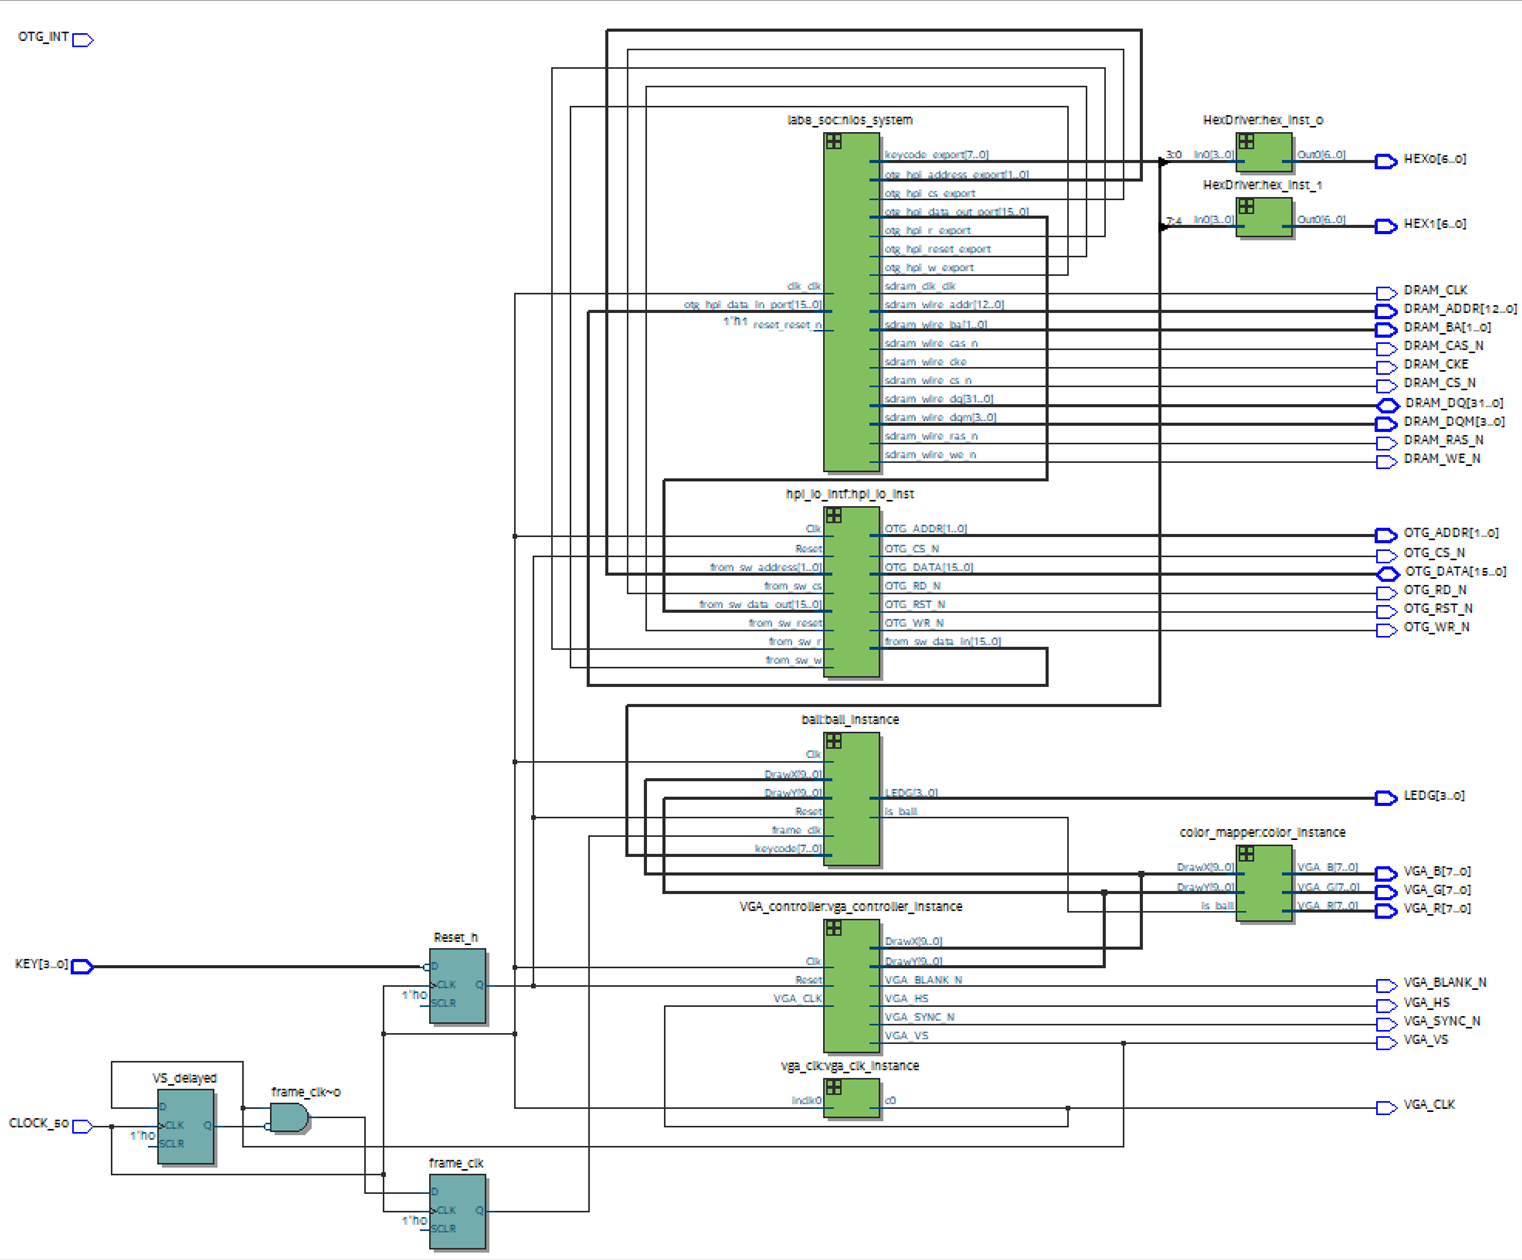
\includegraphics[width=15cm]{toplevel.png}
    \caption{Top level block diagram.}
\end{figure}

\section{Module Description}
\textbf{Module}: lab8.sv \\ 
\textbf{Inputs}: CLOCK\_50, KEY, OTG\_INT \\ 
\textbf{Outputs}: HEX0, HEX1, VGA\_R, VGA\_G, VGA\_B, VGA\_CLK, VGA\_SYNC\_N, VGA\_BLANK\_N, VGA\_VS, VGA\_HS, [1:0] OTG\_ADDR, OTG\_CS\_N, OTG\_RD\_N, OTG\_WR\_N, OTG\_RST\_N, OTG\_INT, [12:0] DRAM\_ADDR, [1:0] DRAM\_BA, [3:0] DRAM\_DQM, DRAM\_RAS\_N, DRAM\_CAS\_N, DRAM\_CKE, DRAM\_WE\_N, DRAM\_CS\_N, DRAM\_CLK, [3:0] LEDG \\
\textbf{Inouts}: [15:0] OTG\_DATA, [31:0] DRAM\_DQ \\
\textbf{Description}: This is the top-level module. \\ 
\textbf{Purpose}: This module instantiates the low-level modules and connect them properly. \\

\textbf{Module}: VGA\_controller.sv \\ 
\textbf{Inputs}: Clk, Reset, VGA\_CLK \\ 
\textbf{Outputs}: VGA\_HS, VGA\_VS, VGA\_BLANK\_N, VGA\_SYNC\_N, [9:0] DrawX, [9:0] DrawY \\
\textbf{Description}: This module controls the VGA signals (horizontal and vertical). \\ 
\textbf{Purpose}: This module keeps tracks of the pixel that is currently under test, so that we can draw that pixel correctly. \\

\textbf{Module}: hpi\_io\_intf.sv \\ 
\textbf{Inputs}: Clk, Reset, [1:0] from\_sw\_address, [15:0] from\_sw\_data\_out, from\_sw\_r, from\_sw\_w, from\_sw\_cs, from\_sw\_reset \\ 
\textbf{Outputs}: [15:0] from\_sw\_data\_in, [1:0] OTG\_ADDR, OTG\_RD\_N, OTG\_WR\_N, OTG\_CS\_N, OTG\_RST\_N \\
\textbf{Inputs}: [15:0] OTG\_DATA \\
\textbf{Description}: This module sends some control signals to the OTG chip. \\ 
\textbf{Purpose}: This module is the hpi interface that communicates with OTG chip, it sends some control signals to the chip. These signals indicate whether to perform a read or write operation, and the address is specified. \\

\textbf{Module}: Color\_Mapper.sv \\ 
\textbf{Inputs}: is\_ball, [9:0] DrawX, [9:0] DrawY \\ 
\textbf{Outputs}: [7:0] VGA\_R, [7:0] VGA\_G, VGA\_B \\
\textbf{Description}: This module determined whether the current pixel should display color. \\ 
\textbf{Purpose}: This module is used to draw the ball, if the current pixel is part of the ball, then it will be colored, and if not, it will remain the background color. \\

\textbf{Module}: ball.sv \\ 
\textbf{Inputs}: Clk, Reset, frame\_clk, [9:0] DrawX, [9:0] DrawY, [7:0] keycode \\ 
\textbf{Outputs}: is\_ball, [3:0] LEDG \\
\textbf{Description}: This module determines whether the current pixel is part of the ball, and it is also in charge of changing the motion direction according to the given keycode. \\ 
\textbf{Purpose}: This module indicates whether the current pixel is part of the ball. It also memorizes the motion direction of the ball, and it will change direction according to the keycode. Moreover, it handles the case when the ball is bouncing back. \\

\begin{figure}[H]
    \centering
    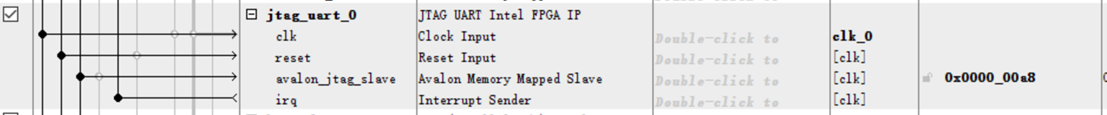
\includegraphics[width=16cm]{JTAG_UART.png}
    \caption{JTAG\_UART.}
\end{figure}
This module allows us to use the terminal of the host computer to communicate with the NOIS using print and scan statements in C.

\begin{figure}[H]
    \centering
    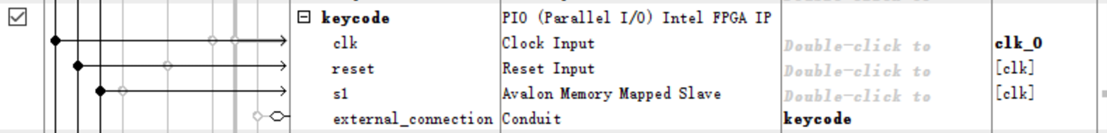
\includegraphics[width=16cm]{keycode.png}
    \caption{Keycode.}
\end{figure}
This module outputs the keycode from USBRead.

\begin{figure}[H]
    \centering
    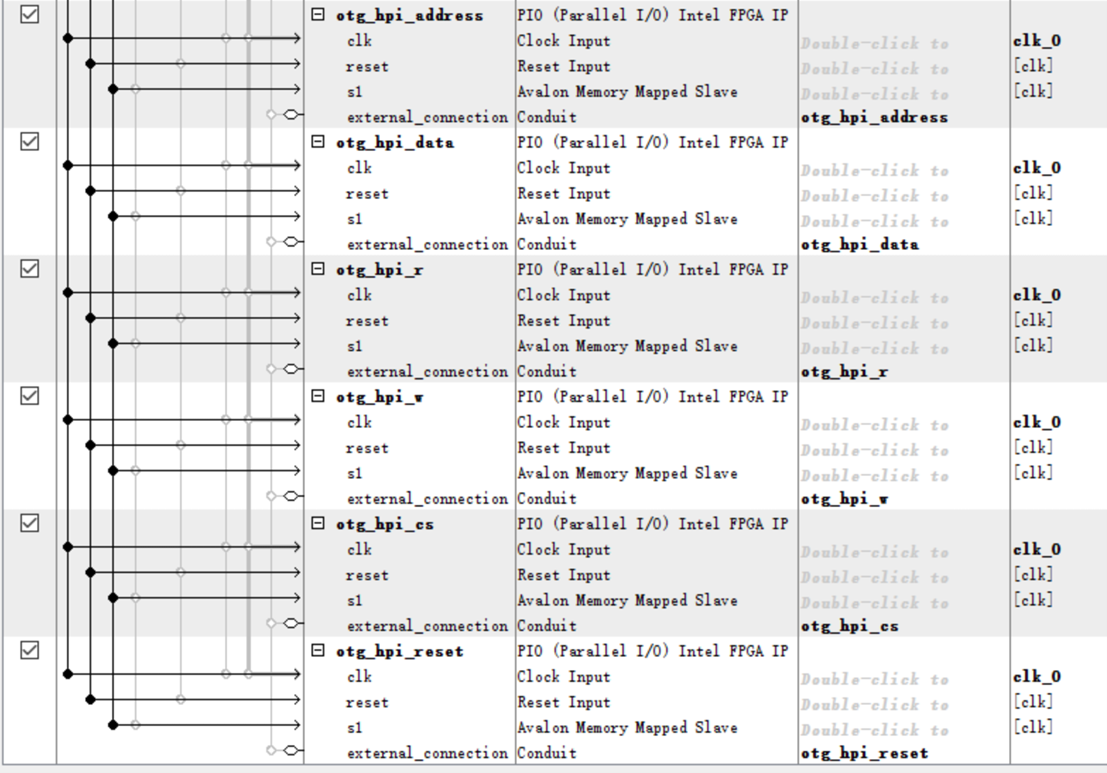
\includegraphics[width=16cm]{otg.png}
    \caption{Otg\_hpi interface.}
\end{figure}
This module is the otg\_hpi interface signals. All of them except hpi\_data are output signals from Nios. Hpi\_data is inout signal which transfer data between Nios and USB chip. Hpi\_address is used to specify the desired hpi register. Hpi\_r indicates read operation, hpi\_w indicates write operation and hpi\_cs indicates chip select. Hpi\_reset is used to reset.

\section{Answers to Both Hidden Questions}
Question: What are the advantages and/or disadvantages of using a USB interface over PS/2 interface to connect to the keyboard? List any two. \\

Answer: The USB interface only accepts 6 keypresses at once while the PS/2 interface has no such limit. For USB devices to send information to the host device, they wait for the host to continuously request polls. While the PS/2 devices send interrupt signals to pause the CPU and send information. \\

Question: Notice that Ball\_Y\_Pos is updated using Ball\_Y\_Motion. Will the new value of Ball\_Y\_Motion be used when Ball\_Y\_Pos is updated, or the old? What is the difference between writing ``Ball\_Y\_Pos\_in = Ball\_Y\_Pos + Ball\_Y\_Motion;" and ``Ball\_Y\_Pos\_in = Ball\_Y\_Pos + Ball\_Y\_Motion\_in;"? How will this impact behavior of the ball during a bounce, and how might that interact with a response to a keypress? \\

Answer: Old motion is used. ``Ball\_Y\_Pos\_in = Ball\_Y\_Pos + Ball\_Y\_Motion;" updates the position with the old motion, while ``Ball\_Y\_Pos\_in = Ball\_Y\_Pos + Ball\_Y\_Motion\_in;" updates the position with the new motion. If we use the latter one, the ball will change the direction as soon as it hits the boundary or takes in a keypress but if we use the former one, the ball will go along the direction before until the next period (rising edge of the clock signal). \\

\section{Answer to Post Lab Questions}
Question: What is the difference between VGA\_clk and Clk? \\

Answer: Clk is 50 MHz clock and VGA\_clk is 25 MHz clock. Clk is the clock for the NIOS-II processor and its PIOs, while the VGA\_clk is for the screen refreshing pixel by pixel (1/25MHz=4ns to update one pixel). \\

Question: In the file io\_handler.h, why is it that the otg\_hpi\_data is defined as an integer
pointer while the otg\_hpi\_r is defined as a char pointer? \\

Answer: The otg\_hpi\_r stores the read enable signal. There is only 1 or 0 so char (1 byte) is enough. The otg\_hpi\_data stores the data we read or write so int type will be better. \\

\begin{table}[H]
    \centering
    \resizebox*{8cm}{5cm}{
        \begin{tabular}{|l|l|l|l|}
        \hline
        LUT           & 2696            \\ \hline
        DSP           & 10              \\ \hline
        BRAM          & 55296           \\ \hline
        Flip-Flop     & 2234            \\ \hline
        Frequency     & 100.77MHz       \\ \hline
        Static Power  & 105.16mW        \\ \hline
        Dynamic Power & 1.07mW         \\ \hline
        Total Power   & 177.37mW        \\ \hline
        \end{tabular}
    }
    \caption{Design statistics table for the multiplier.}
\end{table}

\section{Conclusion}
\subsection{Functionality}
Both the hardware and software worked fine. The ball can be controlled by our instructions through the keyboard. However, when we went to the laboratory and used the keyboard there, we encountered some weird warnings and the NIOS-II stopped taking in the keycode after we pressed the KEY[0] to reset. Later, we changed a keyboard and everything worked fine as before. We considered it to be the keyboard hardware problem but we do not understand the specific reason.

\subsection{About the Lab Manual}
We hope to get more information about the connection and how signals transfer between EZ-OTG, NIOS-II, HPI, CY7 and FPGA.

\newpage
\bibliography{}
\bibliographystyle{ieeetr}
\end{document}